\documentclass[18pt]{beamer}
\mode<presentation>{
    \usetheme{WM}
    \usefonttheme{serif}
    \setbeamertemplate{caption}[numbered]
}
\usepackage{amsmath,amsfonts,amssymb,eulervm,xspace}
\usepackage{amsmath,amsfonts,amssymb}
\usepackage{graphicx}
\usepackage{tikz}
\usepackage{subcaption}
\graphicspath{{figures/}}
\usepackage[orientation=landscape,size=custom,width=70,height=40,scale=.6]{beamerposter}
\usepackage[%
    style=phys,%
    articletitle=false,biblabel=brackets,%
    chaptertitle=false,pageranges=false,%
    doi=false,maxnames=2,minnames=1,eprint=false%
  ]
{biblatex}
\addbibresource{library.bib}
\makeatletter
\renewcommand{\@makefnmark}{\makebox{\normalfont[\@thefnmark]}}
\renewcommand\@makefntext[1]{%
    {{\normalfont[\@thefnmark]}\enspace #1}
  }
\makeatother
%\renewcommand{\cite}[1]{[\footfullcite{#1}]}
\renewenvironment{equation}
    {
    \begin{equation*}
    }
    { 
    \end{equation*}
    }

\newcommand{\e}{\vec e}
%-- Header and footer information ----------------------------------
\newcommand{\footleft}{https://scholarworks.wm.edu/honorstheses/1621}
\newcommand{\footright}{snthomas01@email.wm.edu}
\title{Topology of the $O(3)$ non-linear sigma model under the gradient flow}
\author{Stuart Thomas\inst{1} \quad Christopher Monahan\inst{1,2}}
\institute{\inst{1} William \& Mary \quad \inst{2}Jefferson Lab}
%-------------------------------------------------------------------


%-- Main Document --------------------------------------------------
\begin{document}
\begin{frame}{}
  \begin{columns}[t]

    %-- Column 1 ---------------------------------------------------
    \begin{column}{0.32\linewidth}
        \begin{block}{Abstract}
            The $O(3)$ non-linear sigma model (NLSM) is a prototypical field theory for QCD and ferromagnetism, featuring topological qualities. {\bf Though the topological susceptibility $\chi_t$  should vanish in physical theories, lattice simulations of the NLSM find that $\chi_t$ diverges in the continuum limit. \cite{bietenholz2018, berg1981}} We study the effect of the gradient flow on this quantity using a Markov chain Monte Carlo method, finding that a logarithmic divergence persists. This result supports a previous study and indicates that either the definition of topological charge is problematic or the NLSM has no well-defined continuum limit. We introduce a $\theta$-term and analyze the topological charge as a function of $\theta$ under the gradient flow for the first time.
        \end{block}
        \begin{block}{Non-Linear $\sigma$ Model}
            We study the $O(3)$ non-linear sigma model (NLSM) in 1+1 dimensions, defined by the Euclidean action
            \begin{equation*}
                \label{eq:nlsm euclidean action}
                S_E = \frac{\beta}{2} \int d^2x \; \left[ \left(\partial_t \e\, \right)^2+ \left( \partial_x \e\,\right)^2 \right]
            \end{equation*}
        where
        \begin{itemize}
            \item $\e$ is 3-component real vector constrained by $|\e\,|=1$.
            \item $\beta$ is the inverse coupling constant.
            %\item<3-> Applications
                %\begin{itemize}
                    %\item Prototypical model for strong nuclear force
                    %\item Models Heisenberg ferromagnets
                    %\item Applications to string theory
                %\end{itemize}
            %\item<4-> Merits 
                %\begin{itemize}
                    %\item mass gap
                    %\item asymptotic freedom
                %\end{itemize}
        \end{itemize}

        \end{block}

        \begin{block}{Topology of 1+1 $O(3)$ NLSM}
            \begin{columns}
            \begin{column}{0.6\textwidth}
            \begin{enumerate}
                \item Since the Lagrangian must disappear as $x \rightarrow \infty$, the field $\e$ becomes uniform.
                \item Therefore, we can envision 1+1 spacetime as a sphere.
                \item The NLSM field $\e$ becomes mapping between two Riemann spheres ($S^2 \rightarrow S^2$).
                \item Every configuration has an associated {\bf topological charge} $Q\in\mathbb{Z}$ (see Fig.~\ref{fig:homotopy}).
                \item The ensemble has a {\bf topological susceptibility} $\chi_t \equiv \left(\langle Q^2 \rangle - \langle Q \rangle^2\right)/L^2$ which should disappear in the continuum limit.
            \end{enumerate}
            \end{column}
            \begin{column}{0.3\textwidth}
            \begin{figure}
                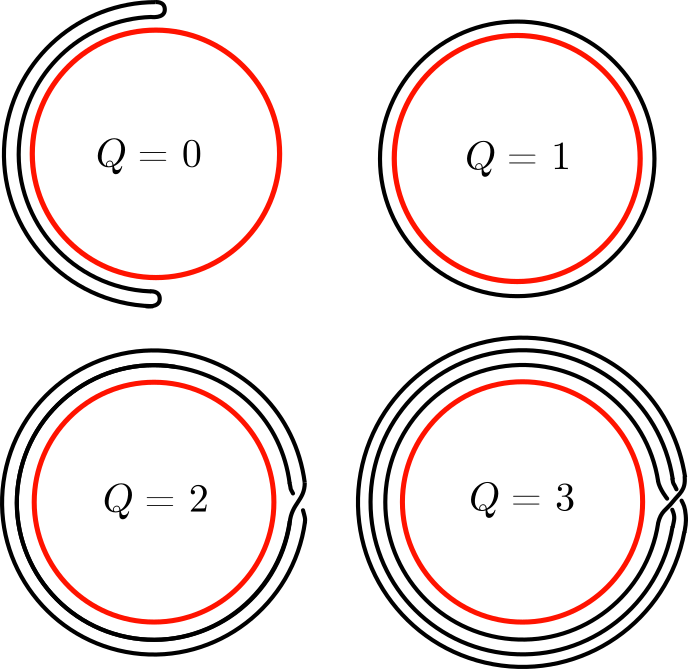
\includegraphics[width=0.9\textwidth]{homotopy.png}
                \caption{\label{fig:homotopy} Visualization of homotopy group of $S^1\rightarrow S^1$}
            \end{figure}
            \end{column}
            \end{columns}
        \end{block}

        \begin{block}{The Gradient Flow}
        \begin{itemize}
            \item Successful in removing $\chi_t$ divergence in QCD by reducing ultraviolet divergences.
            \item Introduces a new dimension, $\tau$, called the ``{\bf flow time},'' which pushes fields towards action minima 
            %\item For NLSM, we use a fourth-order Runge-Kutta to approximate the flow.
        \end{itemize}
        \begin{figure}[h]
          \centering
          \def \Width {0.14\textwidth}
              \begin{subfigure}[b]{\Width}\centering
                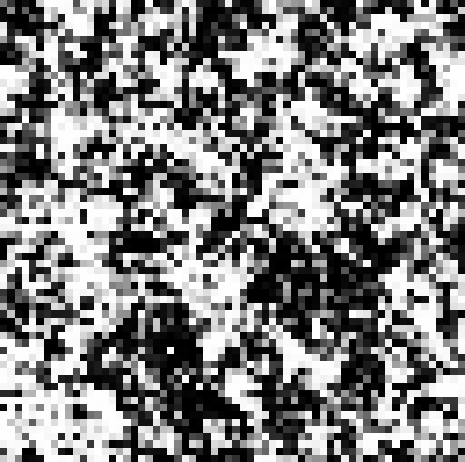
\includegraphics[width=0.9\textwidth]{gf0.png}
                \caption{$\tau=0$}
              \end{subfigure}%
              \begin{subfigure}[b]{\Width}\centering
                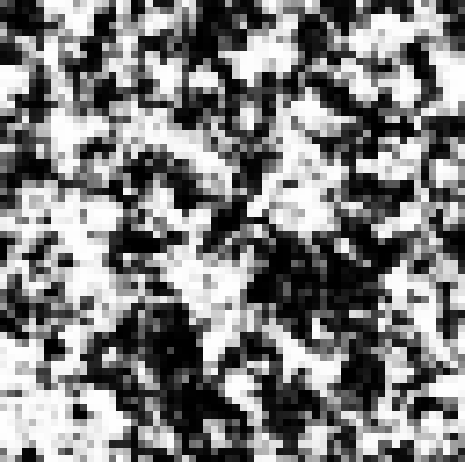
\includegraphics[width=0.9\textwidth]{gf1.png}
                \caption{$\tau=0.001$}
              \end{subfigure}%
              \begin{subfigure}[b]{\Width}\centering
                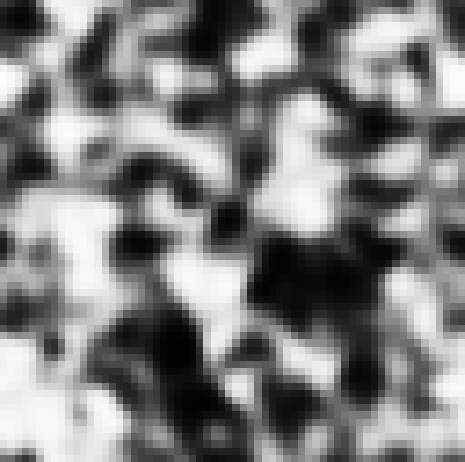
\includegraphics[width=0.9\textwidth]{gf2.png}
                \caption{$\tau=0.01$}
              \end{subfigure}%
              \begin{subfigure}[b]{\Width}\centering
                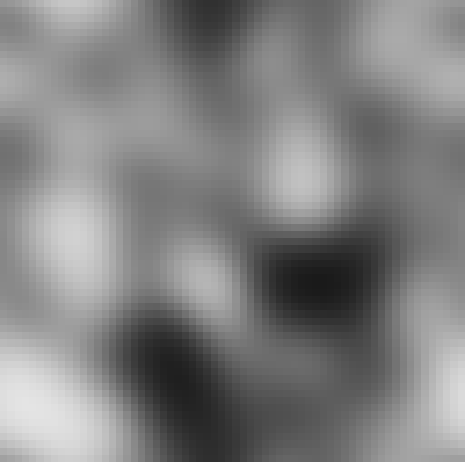
\includegraphics[width=0.9\textwidth]{gf3.png}
                \caption{$\tau=0.1$}
              \end{subfigure}%
              \caption{\label{fig:flow} Visualization of gradient flow in $\phi^4$ model}
        \end{figure}
        \end{block}
    \end{column}%1
    \begin{column}{0.32\linewidth}
        %\begin{block}{Research Question}
            %{\bf Can the gradient flow remove the topological susceptibility divergence in the NLSM?}
        %\end{block}

        \begin{block}{Computational Method}
            We generate lattice field configurations with a Markov Chain Monte Carlo method
            \begin{itemize}
                \item Metropolis algorithm on each site, forming a ``{\bf sweep}'' of the lattice.
                \item Wolff cluster algorithm every five Metropolis sweeps
                \begin{figure}[h]
                  \centering
                      \begin{subfigure}[b]{0.3\textwidth}\centering
                        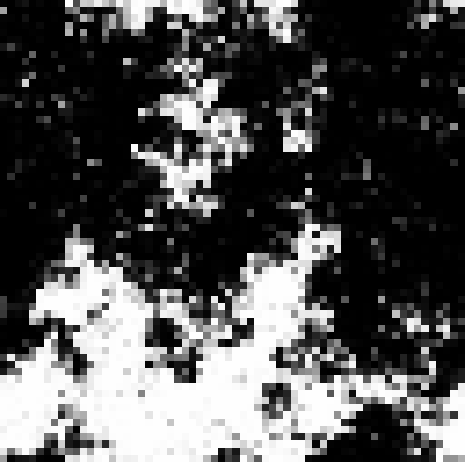
\includegraphics[width=0.5\textwidth]{wolffa.png}
                        \caption{before cluster flip}
                      \end{subfigure}%
                      \begin{subfigure}[b]{0.3\textwidth}\centering
                        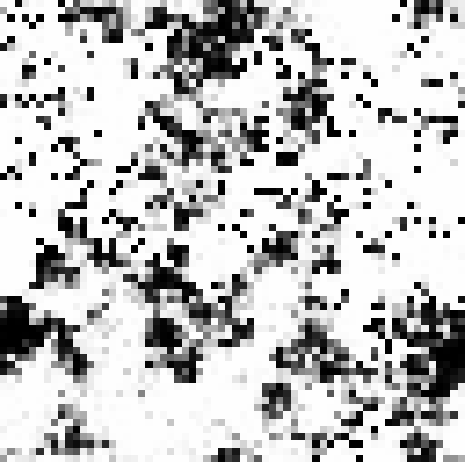
\includegraphics[width=0.5\textwidth]{wolffb.png}
                        \caption{after cluster flip}
                      \end{subfigure}
                      \hfill
                      \caption{\label{fig:wolff} Visualization of Wolff cluster algorithm in $\phi^4$ model}
                \end{figure}
                 \item Thermalize with 1,000 sweeps
                \item Sample every 50 sweeps to reduce autocorrelation
            \end{itemize}
            %\hline
            
            The ensemble has a topological susceptibility $\chi_t \equiv \left(\langle Q^2 \rangle - \langle Q \rangle^2\right)/L^2$ which should disappear in the continuum limit.
        \end{block}
        

        \begin{block}{Topological Charge on the Lattice}
            %Following Berg \& L\"usher~\footfullcite{berg1981}, define topological charge density $q(x^*)$ for each plaquette $x^*$ such that
            Following~\cite{berg1981}, we define topological charge density $q(x^*)$ for each plaquette $x^*$ such that
            \begin{equation}
                Q = \sum_{x^*} q(x^*)
            \end{equation}
            \begin{equation}
                q(x^*) = \frac{1}{4\pi} \bigg[A\Big(\e(x_1), \e(x_2), \e(x_3)\Big) + A\Big(\e(x_1), \e(x_3), \e(x_4)\Big) \bigg].
            \end{equation}
            \begin{figure}[H]
                \begin{subfigure}[b]{0.4\textwidth}
                \centering
                \begin{tikzpicture}[scale=0.8, every node/.style={scale=1.2}]
                    \draw[step=4cm,gray,thin] (-1,-1) grid (5,5);
                    \draw[dotted] (0,0) -- (4,4);
                    \draw[thick](0,0) node[circle,fill,inner sep=0pt, minimum size=0.3cm]{} node[anchor=north west] {$x_1$} -- 
                                (0,4) node[circle,fill,inner sep=0pt, minimum size=0.3cm]{} node[anchor=north west] {$x_2$} -- 
                                (4,4) node[circle,fill,inner sep=0pt, minimum size=0.3cm]{} node[anchor=north west] {$x_3$} -- 
                                (4,0) node[circle,fill,inner sep=0pt, minimum size=0.3cm]{} node[anchor=north west] {$x_4$} -- cycle ;
                                \draw[] (2,2) node[circle,fill,inner sep=0pt, minimum size=0.3cm]{} node[anchor=north east]{$x^*$};


                    \draw[-stealth] (0.2,1) -- (0.2,3);
                    \draw[-stealth] (1,3.8) -- (3,3.8);
                    \draw[-stealth] (3,3.5) -- (1,1.5);

                    \draw[-stealth] (1,0.5) -- (3,2.5);
                    \draw[-stealth] (3.8,3) -- (3.8,1);
                    \draw[-stealth] (3,0.2) -- (1,0.2);
                \end{tikzpicture}
                \caption{a plaquette broken up into two triangles}
                %\caption{\label{fig:plaquette} Visualization of plaquette $x^*$. The dotted line separates the plaquette into two signed areas which are used to define the topological charge density $q(x^*)$. Arrows represent order of signed area.}
                \end{subfigure}
                \begin{subfigure}[b]{0.4\textwidth}
                \centering
                \begin{tikzpicture}[scale=0.7, every node/.style={scale=1}]
                    \pgfdeclarelayer{nodelayer}
                    \pgfdeclarelayer{edgelayer}
                    \pgfdeclareradialshading{sphere4}{\pgfpoint{-0.2cm}{0.5cm}}% 
                        {rgb(0cm)=(1,1,1);
                        rgb(1cm)=(0.5,0.5,0.5); rgb(1.05cm)=(1,1,1)}
                        %rgb(0.7cm)=(0.1,0.1,0.1); rgb(1cm)=(0.5,0.05,0); rgb(1.05cm)=(1,1,1)}
                    \pgfsetlayers{nodelayer,edgelayer}
                    \tikzstyle{label}=[fill=none, draw=none, shape=circle]
                    \tikzstyle{point}=[inner sep=0pt, minimum size=0.2cm,fill=black, draw, shape=circle]
                    %\tikzstyle{interior line}=[{Stealth[scale=1.5]}-,dotted,thick]
                    \tikzstyle{interior line}=[dotted,thick]

                    \tikzstyle{triangle}=[thick]
                    \tikzstyle{arrow}=[->, thick]
                    \begin{pgfonlayer}{nodelayer}
                        \node [style=point] (4) at (0.5, 2.5) {};
                        \node [style=point] (5) at (0.55, 0.625) {};
                        \node [style=point] (6) at (2.25, 0.75) {};
                        \node (7) at (0, 0) {};
                        \node (8) at (1.25, 1.375) {};
                        \node (9) at (2.425, 2.525) {};
                    \end{pgfonlayer}
                    \begin{pgfonlayer}{edgelayer}
                        \draw (0,0) circle (3cm);
                        %\shade[inner color=white,outer color=lightgray] (0,0) circle (3cm);
                        \shade[shading=sphere4] (0,0) circle (3cm);
                        \draw [bend left=15,style=triangle] (4.center) to (6.center);
                        \draw [bend left=355,style=triangle] (6.center) to (5.center);
                        \draw [bend right=5,style=triangle] (5.center) to (4.center);
                        \draw [style=interior line] (4.center) to (7.center);
                        \draw [style=interior line] (5.center) to (7.center);
                        \draw [style=interior line] (6.center) to (7.center);
                        \draw [fill=gray!80] (4.center) to [bend left=15] (6.center) to [bend left=355] (5.center) to [bend right=5] cycle;

                        %\draw [style=arrow] (8.center) to (9.center);

                        \node [style=label, anchor=north] at (2.25, 0.75) {\small $\e(x_1)$};
                        \node [style=label, anchor=north] at (0.55, 0.625) {\small $\e(x_2)$};
                        \node [style=label, anchor=east] at (0.5, 2.5) {\small $\e(x_3)$};
                        \node [style=point] at (4){};
                        \node [style=point] at (5){};
                        \node [style=point] at (6){};

                        \node [style=label] at (8) {\small $A$};
                    \end{pgfonlayer}
                \end{tikzpicture}
                \caption{signed area of triangle in target space}
                \end{subfigure}
            \end{figure}

        \vspace{2em}
        {\bf Non-trivial theory}
        \begin{equation*}
            S[\e\,] \rightarrow S[\e\,] - i \theta Q[\e\,].
        \end{equation*}
        A nonzero $\theta$ implies nonzero $\langle Q \rangle$. Furthermore,
        \begin{equation}
            \chi_t \propto \left. \frac{d\,\mathrm{Im}\langle Q \rangle}{d\theta}\right|_{\theta=0}
        \end{equation}
        \end{block}
        \printbibliography
    \end{column}%2
    \begin{column}{0.32\linewidth}

    \begin{block}{$\chi_t$ Divergence}
        \begin{figure}[h!]
            \begin{center}
              \begin{subfigure}[b]{0.45\textwidth}
                  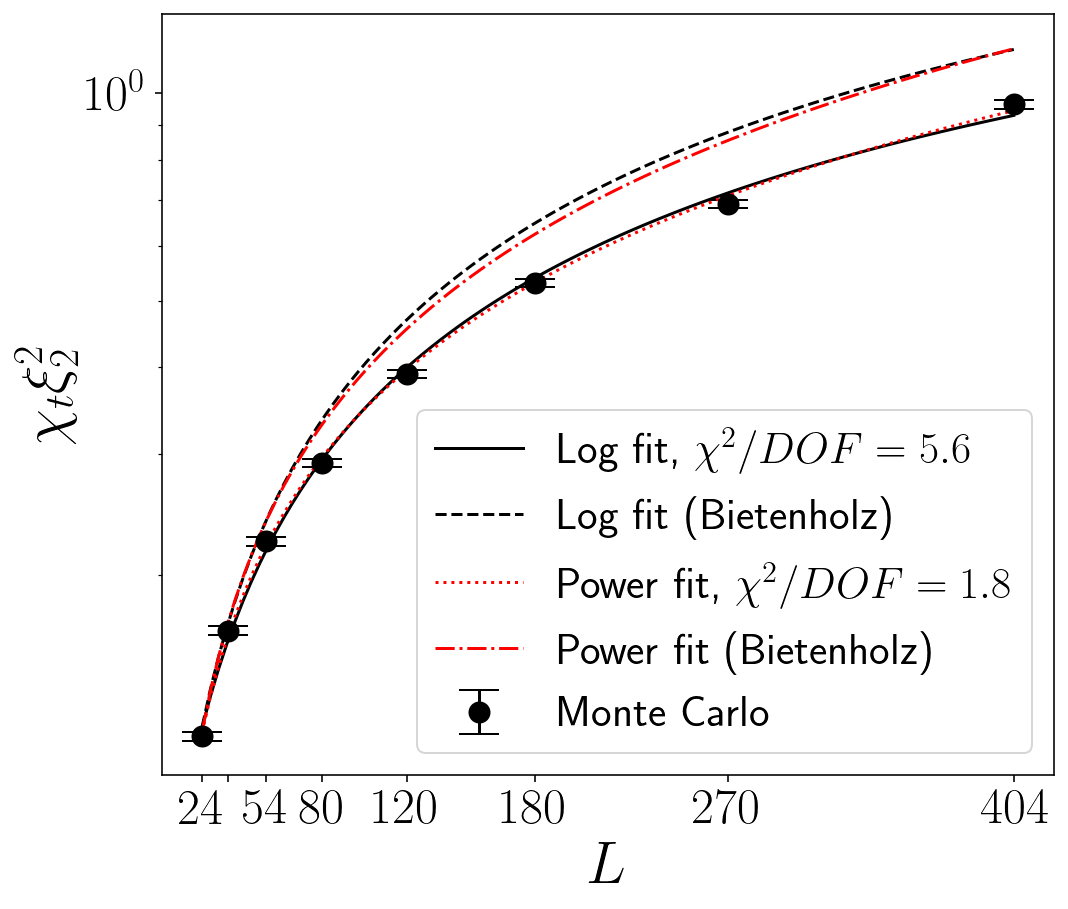
\includegraphics[height=0.7\textwidth]{divergence.png}
                  \caption{$\tau = 0$}
              \end{subfigure}%
              \begin{subfigure}[b]{0.45\textwidth}
                  \centering
                  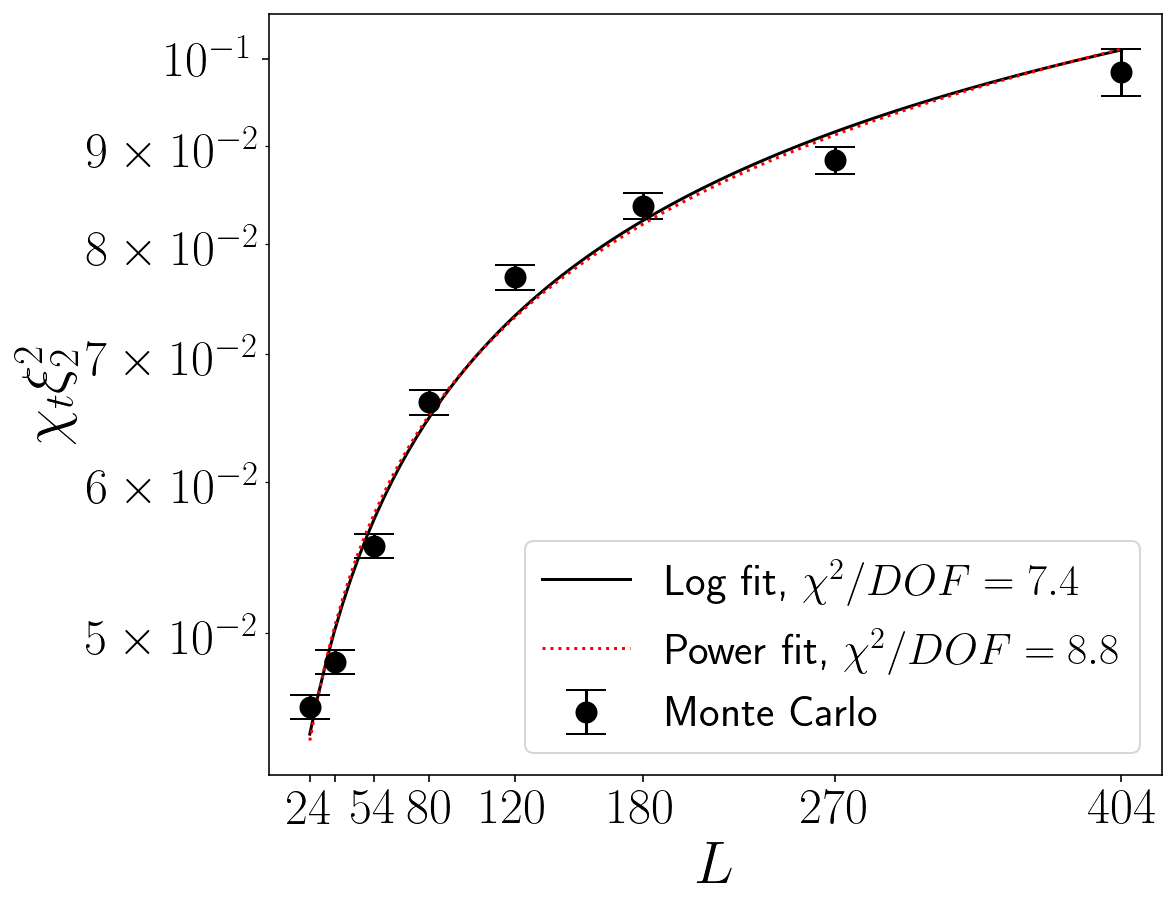
\includegraphics[height=0.7\textwidth]{divergence_flowed.png}
                  \caption{$\tau = 5t_0$}
              \end{subfigure}
            \end{center}
              \caption{\label{fig:divergence} $\chi_t\xi_2^2$ as a function of $L$. $\xi_2$ is the second moment of the correlation function and $t_0$ is a scale-independent unit of flow time. We fit the data with both a logarithmic and power fit. Simulation run with 10,000 measurements every 50 sweeps, 1,000 sweep thermalization. In the $\tau=0$ case, we have compared our result with the curve fits found in \cite{bietenholz2018}.}
              %\caption{Divergent properties with comparison to~\footfullcite{bietenholz2018}, 10,000 measurements}
        \end{figure}
    \end{block}

    \begin{block}{Effect of $\theta$-term on $\langle Q \rangle$}
        \begin{columns}
            \begin{column}{0.35\textwidth}
                Using the path integral formulation, we show that
                \begin{align*}
                    \langle Q \rangle_\theta &=\int \mathcal{D}\e\:Q[\e\,]e^{-S[\e]+i\theta Q[\e]} \\
                                             &=\int \mathcal{D}\e\:\left( Q[\e\,]e^{i\theta Q[\e]} \right) e^{-S[\e]} \\
                                             &=\langle Q e^{i \theta Q} \rangle_{\theta=0}
                \end{align*}
                Therefore, the trivial Monte Carlo method can calculate topological observables, shown in Fig.~\ref{fig:theta}. The increasing slope at $\theta=0$ as $L\rightarrow\infty$ indicates a nonzero suscpetibility in the continuum limit.
            \end{column}

            \begin{column}{0.55\textwidth}
                \begin{figure}[h]
                  \centering
                  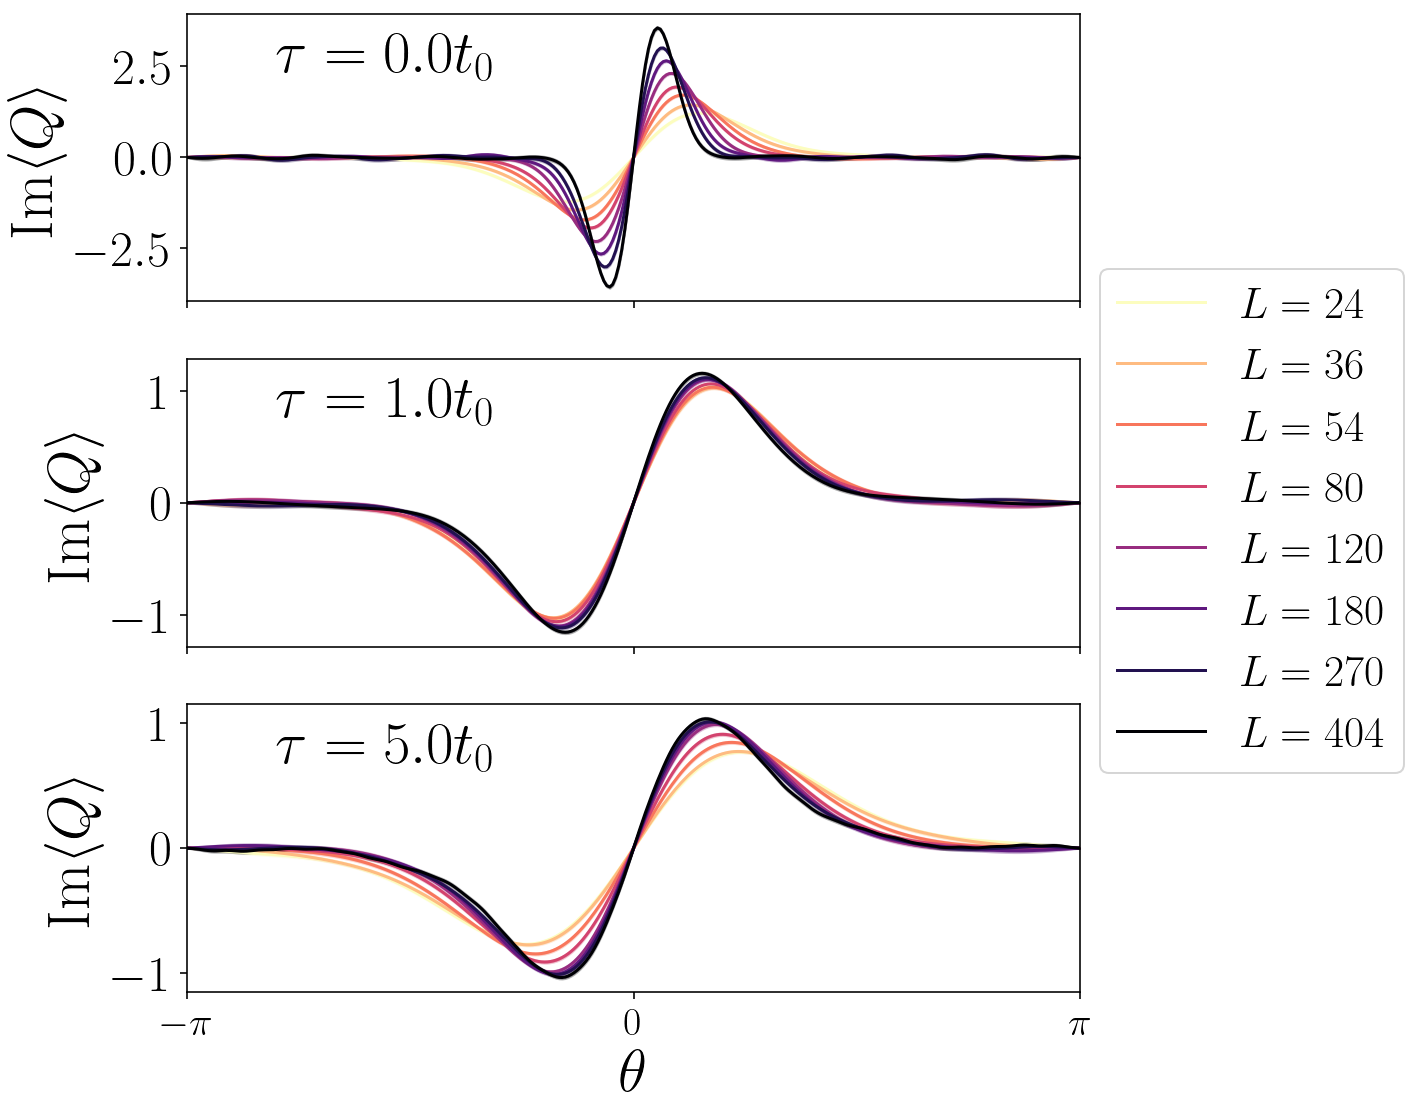
\includegraphics[width=\textwidth]{theta.png}
                  \caption{\label{fig:theta} Nontrivial $\mathrm{Im}\langle Q \rangle$ as a function of $\theta$. Simulation run with 10,000 measurements, every 50 sweeps, 1,000 sweep thermalization. Note the different scaling of the $y$-axis.}
                \end{figure}
            \end{column}
        \end{columns}

    \end{block}

    \begin{block}{Conclusion}
We have studied the topological properties of the 1+1 dimensional NLSM under the gradient flow. Berg \& L\"uscher \cite{berg1981} give three possible sources of divergence:
        {\setlength\parindent{5pt}\begin{enumerate}
                \item ultraviolet modes
                \item the definition of $Q$ on the lattice is problematic
                \item the NLSM has no well-defined continuum limit
        \end{enumerate}}
        Our result supports either options two or three, and requires further work to identify the physical mechanism underlying our results.
    \end{block}

    \end{column}%3


  \end{columns}
\end{frame}
\end{document}
